% TEMPLATE for Usenix papers, specifically to meet requirements of
%  USENIX '05
% originally a template for producing IEEE-format articles using LaTeX.
%   written by Matthew Ward, CS Department, Worcester Polytechnic Institute.
% adapted by David Beazley for his excellent SWIG paper in Proceedings,
%   Tcl 96
% turned into a smartass generic template by De Clarke, with thanks to
%   both the above pioneers
% use at your own risk.  Complaints to /dev/null.
% make it two column with no page numbering, default is 10 point

% Munged by Fred Douglis <douglis@research.att.com> 10/97 to separate
% the .sty file from the LaTeX source template, so that people can
% more easily include the .sty file into an existing document.  Also
% changed to more closely follow the style guidelines as represented
% by the Word sample file. 

% Note that since 2010, USENIX does not require endnotes. If you want
% foot of page notes, don't include the endnotes package in the 
% usepackage command, below.

% This version uses the latex2e styles, not the very ancient 2.09 stuff.

%%%%%%%%%%%%%%%%%%%%%%%%%%%%%%%%%%%%%%%%%%%%%%%%%%%%%%%%%%%%%%%%%%%%%%
%  Packages
%%%%%%%%%%%%%%%%%%%%%%%%%%%%%%%%%%%%%%%%%%%%%%%%%%%%%%%%%%%%%%%%%%%%%%
\documentclass[letterpaper,twocolumn,10pt]{article}
\usepackage{usenix,epsfig,endnotes}
\usepackage{url}
\usepackage{multirow}
\usepackage{booktabs}
\usepackage{color}
\usepackage[normalem]{ulem} 

\newcommand{\urlwofont}[1]{\underline{\urlstyle{same}\url{#1}}}

\newif\ifrev
%%%%%%%%%%%%%%%%%%
% COMMENT OUT NEXT LINE TO HIDE TODOs
\revtrue
%%%%%%%%%%%%%%%%%%
\ifrev
  \newcommand{\yanyan}[1]{{\color{blue} [Yanyan: #1]}}
  \newcommand{\cappos}[1]{{\color{red} [Justin: #1]}}
  \newcommand{\todo}[1]{{\color{red} [todo: #1]}}
  \newcommand{\linda}[1]{{\color{magenta} [Linda: #1]}}
\else
  \newcommand{\yanyan}[1]{}
  \newcommand{\cappos}[1]{}
  \newcommand{\todo}[1]{}
  \newcommand{\linda}[1]{}
\fi


\begin{document}


%don't want date printed
%\date{}


%%%%%%%%%%%%%%%%%%%%%%%%%%%%%%%%%%%%%%%%%%%%%%%%%%%%%%%%%%%%%%%%%%%%%%
%  Title and Authors
%%%%%%%%%%%%%%%%%%%%%%%%%%%%%%%%%%%%%%%%%%%%%%%%%%%%%%%%%%%%%%%%%%%%%%


%make title bold and 14 pt font (Latex default is non-bold, 16 pt)
\title{Quantifying and Minimizing the Risk of Kernel Exploitation}

%for single author (just remove % characters)
\author{
%{\rm Yiwen Li}\\
% Your Institution
%\and
{\rm Yiwen Li, Ali Gholami, Yanyan Zhuang, Justin Cappos}\\\\
New York University, KTH Royal Institute of Technology, UBC \\
\{liyiwen, yyzh, jcappos\}@nyu.edu, gholami@kth.se
% copy the following lines to add more authors
% \and
% {\rm Name}\\
%Name Institution
} % end author


\maketitle


% Use the following at camera-ready time to suppress page numbers.
% Comment it out when you first submit the paper for review.
%\thispagestyle{empty}


%%%%%%%%%%%%%%%%%%%%%%%%%%%%%%%%%%%%%%%%%%%%%%%%%%%%%%%%%%%%%%%%%%%%%%
%  Sections
%%%%%%%%%%%%%%%%%%%%%%%%%%%%%%%%%%%%%%%%%%%%%%%%%%%%%%%%%%%%%%%%%%%%%%


\begin{abstract}

An Operating System (OS) kernel is a trusted part of modern computer systems, 
yet despite substantial effort, kernels still contain bugs and are vulnerable to many types of 
attacks. Many previous approaches, including OS virtualization, system call filtering, and library 
OSes, have been deployed to provide better security. 
However, bugs continue to exist and remain exploitable even with these approaches in place. 

In this paper, we quantitatively measure and evaluate different lines of code in the kernel 
based upon how often these lines are executed within popular applications. 
Analyzing a history of Linux kernel flaws, we propose our �commonly� executed code metric 
and show that it has a strong correlation with being bug-free. 
Our metric provides insights into how to design a security system to provide stronger security 
to computer systems. 
For example, we used our metric to come up with a design that minimizes the trust placed 
in risky privileged code. This is done by containing, within a sandbox, risky code that is needed 
to support legacy programs. The sandbox is built so that it has a small TCB that minimizes 
the use of risky code in the kernel. Using this technique, we implemented a sandbox we call Lind. 
By running popular Linux packages and legacy programs inside Lind, we evaluated the 
kernel traces that were generated and compared them against kernel traces produced 
when running programs in environments other than Lind, such as Graphene and VirtualBox. 
Our evaluation demonstrates that designs, such as our Lind prototype, provide security benefits 
by minimizing the use of code that is not commonly executed.

\end{abstract}
\section{Introduction}
\label{sec.introduction}

Privileged code is an essential component of modern computer systems but 
presents a number of security challenges. The privileged code itself is vulnerable 
to attacks and other parts of a system could be damaged when vulnerabilities in 
that privileged code are exploited.

Failures in the TCB allow more impactful crashes (complete system failures), privilege escalation, etc.
(Mention zero-days, impact, etc.)
Decreasing the feasibility of exploitation of the kernel bugs, especially privilege escalation, 
would be a substantial step toward stronger security for computer systems.

Bugs in operating system kernels have motivated development of a diverse set of
technologies to attempt to reduce these risks, such as OS virtualization, system
call filtering, library OSes, etc. Unfortunately, these technologies also 
harbor vulnerabilities that are also exploitable. Even with these technologies in place,
applications from the user space could still have access to a portion of the kernel that might contain 
bugs and is risky to be exposed. 

One contributing factor to security problems associated with these existing technologies and potential
new designs is that it is still unknown which portions of the privileged code are
safe to expose, and which portions would be be vulnerable. 
One key missing puzzle is a standard for quantifying the safety (or risky) levels of the privileged code. 
For example, is it good practice to minimize \textit{the number of lines of code}? cite[?] 
Is \textit{the number of API calls} a good metric for security? cite[Bascule]   
To our best knowledge, there is no quantitative metric to evaluate the privileged code and provide 
insights into how to design a secure system that only interact with the privileged code in a safe way.

In this paper, we provide a quantitative measure that shows
certain areas of privileged code are likely to have flaws.  
The measure examines lines of privileged code that are executed by popular 
programs. The intuition behind this metric is that kernel code 
that is rarely executed is less likely to be rigorously tested and is thus more likely to contain bugs. 
We examine 40 historical  kernel bugs from Linux over the past 5 years and find out that 
``commonly'' executed code metric has a strong correlation with being bug-free. 

By optimizing our metric, we devise the \emph{safely-reimplement}
architecture, which minimizes the amount of risky privileged code that is
executed.  
Risky functionality is itself implemented in a sandbox with
a small trusted-computing base (TCB). 
This additional level of sandboxing provides an outlet for risky functionality, without which
legacy programs will not run, while containing security flaws in this code. 

The contributions of this paper are as follows:
\begin{itemize}
\item We proposed a novel metric for evaluating security level of the privileged code. 
Our metric consists of ``commonly'' executed code in the kernel at the level of ``lines of code''. 

\item We quantitatively measured the privileged code using our metric, and labeled certain portions of 
the kernel as ``safe" and certain portions of the kernel as ``risky''.

\item We designed a novel secure architecture that comes from examining and leveraging our metric. 
Using this new architecture, we implemented a sandbox we called Lind, which provides more secure environment
for running legacy applications. 

\item Evaluation shows that implementation of our sandbox Lind only has the potential to trigger 2.5\% of zero-day 
vulnerabilities we examined, while systems built without using our security metric have more chances to trigger 
vulnerabilities. (illustrate with data from running Graphene and Virtualbox)
\end{itemize}
\section{Motivation}
\label{sec.motivation}

The Operating System (OS) kernel is a critical component of the entire computing system, 
yet is not protected properly and very vulnerable under the current security model of existing 
computing systems.

The kernel has to provide an interface to serve the requests from user applications for acquiring 
essential system resources, such as memory, I/O, CPU, and etc. 
All applications running in the system depend on the kernel to provide essential functionality. 

However, the OS kernel is the privileged code that needs to be well protected. Access to the
kernel code should be avoided as much as possible and be conducted in a very careful manner 
if any contact is necessary. Failing to do this would lead to potential exploitation of kernel bugs and 
may lead to serious damage to the entire computing system.  

The OS kernel has always been an appealing target. During the past few years, 
the exploitation of OS kernels has become a very serious problem that remains to be solved, 
in spite of large amount of efforts devoted by researchers and practitioners. 
There were 125 reported vulnerabilities of the Linux kernel, and 215 reported vulnerabilities 
of all kinds of kernels in 2014 \cite{NVD:14}. Admittedly, the exploitation of user-level software 
has become much harder, as recent versions of popular OSes come with numerous protections 
and exploit mitigations. The principle of least privilege is better enforced in user accounts 
and system services, compilers offer more protections against common software flaws, 
and highly targeted applications, such as browsers and document viewers, have started to 
employ sandboxing technique. On the other hand, the kernel has a huge codebase and 
an attack surface that keeps increasing due to the constant addition of 
new features \cite{Metrics:13}. Indicatively, the size of the Linux kernel in terms of lines of code 
has more than doubled, from 6.6 MLOC in v2.6.11 to 16.9 MLOC in v3.10 \cite{Linux:13}.

Opportunities for kernel exploitation are abundant. As an example consider the Linux kernel, 
which has been plagued by common software flaws, such as stack and heap buffer overflows 
\cite{CVE:20093234, CVE:20131828, CVE:20132892}, NULL pointer and pointer arithmetic errors 
\cite{CVE:20050736, CVE:20092698}, memory disclosure vulnerabilities 
\cite{CVE:20093002, CVE:20104073}, use-after-free and format string bugs 
\cite{CVE:20132852, CVE:20134343}, signedness errors \cite{CVE:20103437, CVE:20132094}, 
integer overflows \cite{CVE:20050736, CVE:20102959}, race conditions 
\cite{CVE:20091527, CVE:20093547}, as well as missing authorization checks and 
poor argument sanitization vulnerabilities 
\cite{CVE:20103904, CVE:20104347, CVE:20120946, CVE:20130268}. 
The exploitation of these bugs is particularly effective, 
despite the existence of kernel protection mechanisms, 
due to the weak separation between user and kernel space.

To build a secure computing system, it is critical to provide sufficient protection for the kernel and 
prevent kernel exploitation from happening. Many previous attempts, including OS virtualization, 
system call filtering, library OSes and etc. have tried to address this problem. However, 
kernel exploitation still exist, and the problem has not been solved effectively, which leads to a 
fundamental question, why is it not working and what are we missing? After thinking about this
question and examining previous work, we find that one key missing puzzle is that people do not know 
clearly which part of the kernel are safe and can be exposed without potential dangers. Many previous
work, such as building a sandbox and using library OSes focused on isolating user programs. While isolation 
can be useful and help mitigate the problem, the proposed systems still get access to the kernel. 
And the key is: the way they access the kernel has no difference than before, because they do not 
know what's the best way to leverage the kernel securely. So, essentially, what they are doing is just moving 
the attack surface from the previous place (between the user space and the kernel) to another place 
(between the new proposed system and the kernel). The attack surface doesn't necessarily shrink. 
Therefore, the proposed solutions were not effective. 

It would be more effective, if we can actually shrink the attack surface and have better control over 
the interface exposed by the kernel. In another word, we need to be crystal clear about which portion of 
the kernel is safe and which portion of the kernel is risky. To obtain this piece of critical information, we
propose a novel security metric to quantitatively measure and evaluate the kernel. Our metric will provide
insights into the kernel and let us understand security features of the kernel in a better way. 

With the help from our metric, we would be able to process the power of controlling the interface 
exposed to the user space in a precise and secure way. We can then design and build secure systems 
that provide stronger protection to the kernel. Ideally, we would like to only expose safe portion 
of the kernel to the user space. Realistically, in some cases, even if we have to expose certain risky portion 
of the kernel, we know clearly about the potential dangers and therefore can come up with better 
strategies to mitigate the potential damage. 
\section{Solution: A Quantitative Security Metric}
\label{sec.solution}

We propose a security metric to assess and evaluate the kernel in a quantitative way. 
Our metric focuses on examining the precise lines of code in the kernel that are executed 
when running applications in the user space. We define the \textit{kernel trace} to be the 
set of lines of code in the kernel that are executed by running applications. With the \textit{kernel trace}, 
we are able to determine the \textit{kernel coverage} of running applications. The \textit{kernel coverage} 
refers to the percentage proportion of the \textit{kernel trace} to the entire kernel. 

To determine whether the generated \textit{kernel trace} is safe or risky, we examined 40 historical bugs from
the Linux kernel. We identified the lines of code in the kernel that have the potential to trigger each of the bugs.
We define the lines of code in the kernel that have the potential to trigger bugs as \textit{trap trace}.
We then compare the \textit{kernel trace} against the \textit{trap trace}. If there is correlation between 
them, we label the \textit{kernel trace} as \textit{risky trace}. If there is no correlation found between them, 
we label the \textit{kernel trace} as \textit{safe trace}.

\subsection{The Goal of Our Metric}
We propose our metric to achieve the following goals:
\begin{itemize}
\item Define a standard way to conduct quantitative measurement of the lines of code being executed 
in the kernel. 
\item Use our metric to acquire precise information about the \textit{kernel trace} and \textit{kernel coverage} 
of running different applications, to gain better understanding of which portion of the kernel is reachable and 
reachable by running popular applications. 
\item Determine the \textit{risky trace} and \textit{safe trace} from the \textit{kernel trace} generated by
running a set of different applications. Therefore, construct a picture of the the safe portion and risky portion
of the kernel. 
\end{itemize}

\subsection{Intuition Behind Our Metric}
There are some fundamental questions that we need to answer regarding our metric:
\begin{itemize}
\item \textbf{\textit{Why would you need this new metric?}}
\item \textbf{\textit{How did you come up with this metric?}}
\item \textbf{\textit{Can you prove this metric is useful?}}
\end{itemize}

To answer those questions:
\begin{itemize}
\item \textbf{\textit{Our metric is necessary:}} previously, there are very limited ways to measure the kernel
code, in terms of which portion is executed, let along any quantitative ways. Our metric fills the hole in this 
area, and provide a precise way to conduct quantitative measurement.
\item \textbf{\textit{Our metric is reasonable:}} examining the exact lines of code is fine-grained, and therefore
more precise. It provides insights into what is really going on inside the kernel. 
\item \textbf{\textit{Our metric is useful:}} the data of the \textit{kernel trace} and \textit{kernel coverage}
can provide precise statistics of the reachable kernel, which itself is valuable for gaining better understanding
of the kernel. In addition, the information gained by using our metric can help with new designs that expose 
the kernel in a more secure way. 
\end{itemize}

\subsection{Quantitative Measurement of the Kernel Using Our Metric}
Now, we use the metric that we proposed to conduct quantitative measurement of the kernel. 
To be more precise, we would like to gain the \textit{kernel trace} and \textit{kernel coverage} of running 
different set of applications. We can then determine the reachable kernel and reachable kernel by 
running popular applications. Finally, we compare the \textit{kernel trace} we generated against the 
\textit{trap trace} composed of bugs to label \textit{risky trace} and \textit{safe trace}. 

\subsubsection{\textit{Kernel Trace} and \textit{Kernel Coverage} of basic system calls}
Results with running a set of basic system calls in C program. Results with running the system call fuzzer. 

\subsubsection{\textit{Kernel Trace} and \textit{Kernel Coverage} of using popular applications}

\subsubsection{\textit{Kernel Trace} and \textit{Kernel Coverage} of daily user behavior}

\subsubsection{\textit{Security Analysis of the Kernel}}
Compare the \textit{kernel trace} against the \textit{trap trace}.
Label the \textit{risky trace} and the \textit{safe trace}.
\section{Background}
\label{sec.background}

In this section, we first discuss our threat model. We then give necessary description about the two sandboxing 
techniques that our work depends on. One is Google's Native Client sandbox, the other is Seattle's Repy sandbox. 

\subsection{Threat Model}

In our threat model, threats refer to any behavior that may cause potential harm to the system, 
which may be triggered by malicious code or bugs in non-malicious programs.

In order to fully execute their functions, applications need to have access to a set of privileges provided by 
the operating system, usually exposed as system calls. The primary security goal of a sandbox is to restrict a program 
to some subset of privileges, usually by exposing a set of functions that mediate access to the underlying 
operating system privileges. Threats occur when applications obtain access to privileges that were not intentionally 
exposed by the sandbox, thus escaping the sandbox \cite{Repy:10}.

To pose threats to a sandbox, we assume that applications may use multiple threads to modify visible state or issue 
concurrent requests which may trigger a race condition. Our goal is to prevent bugs in the code from allowing an user 
program to escape the sandbox.


\subsection{Google's Native Client Sandbox}

Google's Native Client (NaCl) is a sandbox for untrusted x86 native code \cite{NaCl:09}. NaCl aims to give applications 
the computational performance of native applications without compromising safety. NaCl uses software fault isolation 
and a secure runtime to direct system interaction and side effects through interfaces managed by NaCl. NaCl provides 
operating system portability for binary code while supporting performance-oriented features, such as thread support, 
instruction set extensions such as SSE, and use of compiler intrinsics and hand-coded assembler. 

We leverage NaCl execution environment. NaCl allows the efficient execution of legacy code in the form of x86 and ARM 
binaries that are built with a lightly modified compiler tool chain.

\subsection{Seattle's Repy Sandbox}

Seattle's Repy is a restricted subset of Python \cite{Repy:10}, which is a sandbox that provides safe environment for running 
applications.

In Lind, we use Repy to safely re-implement a subset of the POSIX API, which provides fundamental operating system 
access to many applications. The POSIX API, which itself is difficult to secure, is constructed using the Seattle's Repy 
sandbox which provides performance isolation and safety. 
\section{Architecture}
\label{sec.architecture}


In this section, we describe the design and architecture of Lind. We explain the choices we made 
and the rationale behind our decision. We also discuss the challenges we are facing.

The primary goal of Lind is to execute untrusted applications in a secure way. To achieve this goal, 
we try to minimize the portion of reachable kernel which might be exposed to applications in the user space. 
Existing system call interface in the kernel is rich and exploitable. We decided to safely re-implement most OS
functionalities in our Repy sandbox. We use Repy sandbox to reconstruct a POSIX interface, which provides 
OS functionalities sufficient for most applications. 
   
When security goal is achieved, we still want to execute applications efficiently, preferably in a light-weight 
way that can reduce potential overhead. We leverage Google's Native Client (NaCl) to achieve
this second goal of efficiency.  

Combining both NaCl and Repy sandbox, we have formed our dual-layer sandbox architecture 
design of Lind. (Shown in Figure 2.)  


\begin{figure}[h]
\centering
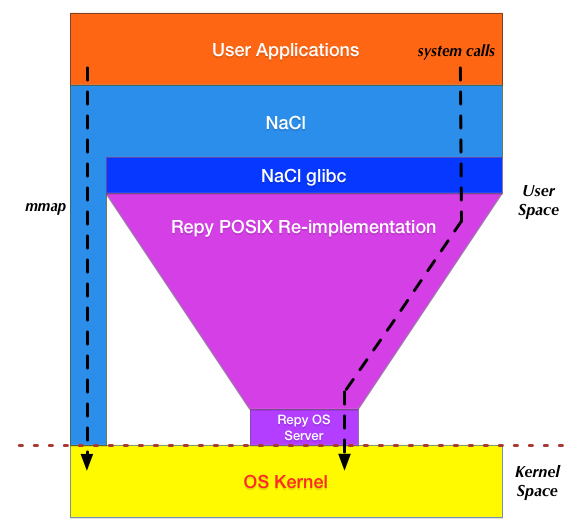
\includegraphics[width=1.0\columnwidth]{diagram/lind_architecture.png}
\caption{Architecture of Lind}
\label{fig:arch}
\end{figure}


To provide native computation and safe access to the system, Lind combines NaCl and Repy. 
Untrusted programs are run in NaCl, but access to all system resources is diverted to our Repy program. 
This program is responsible for accessing the system on behalf of the program, it is called the Lind Library OS. 
Our NaCl sandbox is built on top of our Repy sandbox. To service a system call in NaCl, a server routine 
marshals its arguments into a text string, and sends the call and the arguments to Repy sandbox. 
The Library OS then executes the appropriate system call, marshals the result and returns it back to NaCl. 
The result is eventually returned as the appropriate native type to the calling program. 

Lind is designed to minimize its footprint within the trusted code base (TCB) of these two sandboxes. 
To achieve that, most of the Lind code is run from within the two sandboxes, the modifications to 
the sandboxes themselves (and therefore the TCB) was extremely small. 

The dual-layer sandbox mechanism completes the achievement of the isolation design goals through 
two features. First, the dual-layer sandbox ensures that all code can modify only device state, 
interact with devices, or interact with the outside world through the new trusted operating system interface. 
Secondly, the customizability of the interface ensures that the system can only modify state, interact with 
devices, or interact with the world at a rate and in a manner specified for the application. For example, 
any attempt to send spam or execute a denial of service attack would trigger limits on resource 
consumption and/or allowable addressing, and would be prevented. 

The dual-layer sandbox also makes the construction of Lind simpler. The complex part of Lind is the 
Library OS which runs in Repy. However, Python is a very powerful language, so it significantly simplified 
the construction of Lind. Even though Python is considered ``slow'' by some, the internals of 
an application in Lind are run in NaCl, a very high performance environment. 
This balances the performance of the system, with the ease of implementation and maintenance 
of the Library OS component of Lind. 

Furthermore, this particular design and architecture for sandboxing ensures the programs are portable. 
Programs running inside Lind are written to work against a standard POSIX glibc interface. 
The Lind runtime is strictly user-level and designed to work on many different platforms including Linux, 
Mac OS X and Windows.

Our sandbox also ensures performance isolation. It is used to limit resource consumption, 
both of computational resources (CPU, memory) and external resources (disk I/O and space, 
network bandwidth). The interposed system calls rate limit access and total consumption of 
each class of device on a configurable basis. CPU and memory limits are enforced on 
a per-process basis. 

Finally, this kind of sandboxing ensures that the lightweight goal is met. Overhead for the Lind system 
is low because the sandbox only incurs overhead when there is a system call; Lind uses a native interface 
for execution, allowing CPU-and-memory-intensive applications to run at speeds that are equivalent 
to NaCl and near native speed. 

Regarding our dual-layer sandbox architecture, one fundamental question is: are two sandboxes 
enough and necessary? Why do we only have two sandboxes? If sandboxing provides more security, 
why not sandbox Repy sandbox's TCB and get more security? The answer to that question is: 
the lowest level sandbox eventually must have some fundamental yet limited access to system resources, 
such as memory, storage, threads, etc. So having multiple sandboxes is not necessary, and two sandboxes in 
our design would be enough. But are two sandboxes indeed necessary? Why not just have one sandbox 
that solves everything? The answer is that the kernel interface is extremely rich and hard to protect. 
In order to have minimal tough into the kernel, as well as provide sufficient API for legacy applications, 
we need to have more than one sandbox to complete the job. One sandbox focuses on protecting 
the kernel and providing POSIX API, the other sandbox deals with executing applications efficiently. 
That is the reason for us to have at least two sandboxes.  

The key point in our design is to achieve safe re-implementation of OS functionalities. 
However, our safe re-implementation has limitations. There are a few functionalities that 
we currently cannot re-implement in our sandbox. Those functionalities include brk, mmap, and threads creation.
\section{Evaluation}
\label{sec.evaluation}


\begin{table*}[t]
\begin{tabular*}{\textwidth}{c @{\extracolsep{\fill}} rrrr}
%\begin{tabular}{lllr}
\toprule
\multicolumn{4}{c}{Kernel Footprint Generated by Running Apache} \\

%\multicolumn{1}{c}{\multirow{2}{*}{Powers} } &
\midrule
 & Native Linux    &  Lind & Graphene \\
\cmidrule(r){2-4}
& \multicolumn{3}{c}{Line Coverage} \\
\midrule
1. arch/x86/include/asm                 & 31.6\%          & 28.0\%    & 30.0\%      \\
2. arch/x86/include/asm/trace    &  10.0\%          & 0.0\%       &  5.0\%       \\
3. arch/x86/kernel                            &  22.8\%          & 19.5\%       & 15.2\%       \\
4. include/net                                     &  2.3\%            & 1.0\%       &  1.5\%          \\
5. drivers/cpuidle/governors         &  68.5\%          & 40.8\%       &  55.2\%       \\
\bottomrule
\end{tabular*}
\caption {Kernel Footprint Coverage}
\label{table:kernel_footprint_coverage}
\end{table*}


Our ultimate goal is to run legacy applications in Lind efficiently and securely. Especially, we want to demonstrate that by 
adopting our new ``safely re-implement'' model, Lind provides stronger security than existing systems using 
``check-and-pass-through'' or ``re-implement'' approaches. 


Through our evaluation, we want to show that:
\begin{itemize} 
  \item Legacy applications can run in Lind with acceptable overhead.
  \item Applications running in Lind can only trigger limited portion of the kernel and only touch commonly used kernel paths.   
  \item In Lind, the lines of code touched in the kernel are commonly used and not likely to trigger kernel bugs.   
\end{itemize}


\subsection{Performance Evaluation}

First, we have run different legacy applications in Lind to test performance overhead. Figure 3. shows the running time 
overhead of executing primes, grep and wget applications. 


\begin{figure}[h]
\centering
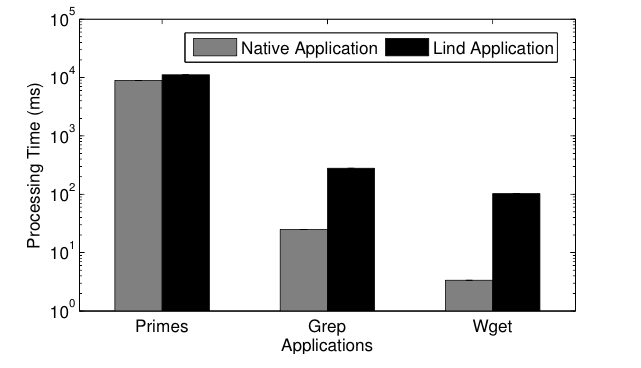
\includegraphics[width=1.0\columnwidth]{diagram/evaluation_01.png}
\caption{Primes, grep and wget performance: native vs. Lind}
\label{fig:arch}
\end{figure}


We have also run Tor in Lind and conducted measurement of performance overhead using Tor's built in benchmarks. 
The results are shown in Figure 4.


\begin{figure}[h]
\centering
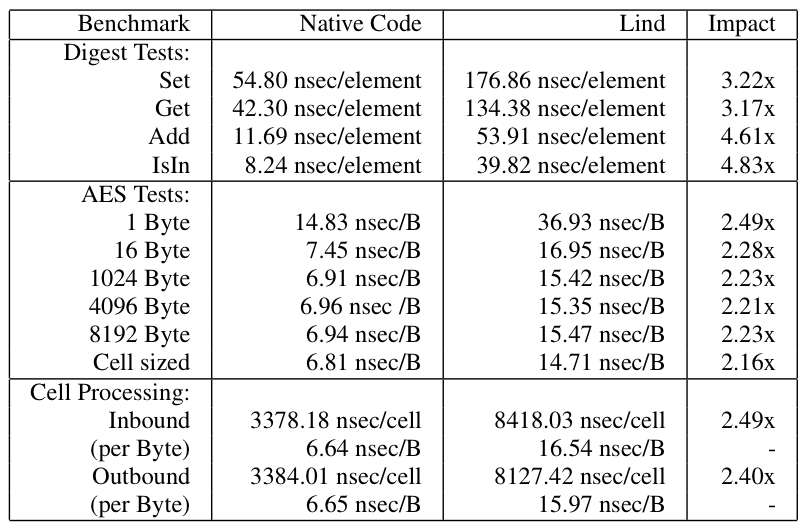
\includegraphics[width=0.9\columnwidth]{diagram/evaluation_02.png}
\caption{Results from Tor's built in benchmark program}
\label{fig:arch}
\end{figure}


To quantify the impact Lind has on memory use, we track how much memory Lind uses versus how much memory 
the same native program uses. Figure 5. shows the peak memory usage for each of the programs.

Lind's memory usage is actually very similar to the native programs, except for an relatively constant additional 
amount of memory (approximately 30 MB). That 30 MB is comprised of the additional overhead of running the NaCl 
sel\_ldr process to run the program, 


To summarize, the above experiments demonstrated that Lind was able to run applications with reasonable time and 
space overhead. Therefore, we believe Lind has the potential to become a widely deployed practical tool for 
common users. 


\begin{figure}[h]
\centering
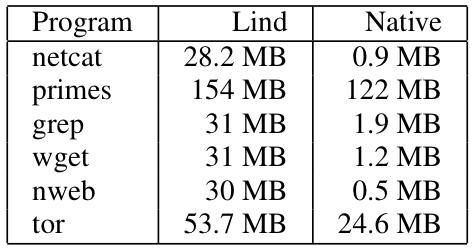
\includegraphics[width=0.6\columnwidth]{diagram/evaluation_03.png}
\caption{Memory consumption of programs running in Lind and natively.}
\label{fig:arch}
\end{figure}


\subsection{Security Evaluation}

In this security evaluation section, we would like to demonstrate the critical advantage of ``safely re-implement" model, 
and show how our design and implementation of Lind benefit from adopting this new isolation model. 
The essential advantages and benefits are better isolation between user applications and the kernel, and stronger 
protection of the kernel. 

The above advantages of Lind are demonstrated through the following facts, supported by our evaluation experiments:

\begin{itemize}  
  \item Only very limited portion of the kernel would be triggered and exposed.   
  \item The lines of code touched in the kernel are commonly used.  
  \item The kernel footprint generated by running applications in Lind is less likely to trigger kernel bugs. 
\end{itemize}

In addition, in order to show that Lind works better than existing system, in this security evaluation section, we also compared 
Lind against Graphene library OS system \cite{Graphene:14} to evaluate their security features. 


\subsubsection{Quantitative Analysis of the Kernel Footprint}

First of all, we want to examine the size of the kernel footprint generated by running applications under different environment.
To be specific, we ran legacy application, Apache, under: 

\begin{itemize} 
  \item Case 1: Native Linux OS
  \item Case 2: Lind
  \item Case 3: Graphene
\end{itemize}

We have quantitatively evaluated the size of the reachable kernel triggered by running applications in both Lind and Graphene, 
and under native linux OS.

The results for running Apache under the three different environment are illustrated in Table \ref{table:kernel_footprint_coverage} 
(speculative data).
 
In this experiments, we choose critical kernel paths and compare the coverage of kernel code under three different 
environment.
As shown from the results, we can learn that for those critical kernel paths, Lind covers only limited portion of the kernel code, 
significantly smaller than the code coverage under native Linux system. This demonstrates that Lind has minimum contact 
with the kernel while running complex legacy applications. Therefore, Lind provides better isolation between untrusted user 
applications and the privileged kernel. 


\subsubsection{Further Analysis of Kernel Footprint Composition}

In the previous subsection, we have quantitatively evaluated the size of kernel footprint generated by running applications 
under native Linux OS, Lind, and Graphene. We have shown that Lind touched the smallest portion of the kernel. 
Next, we want take one step further to closely examine the exact composition of the kernel footprint being touched. 

When we look at the kernel code/path, we can see they are used by different functions and are triggered with 
different frequencies. 
In order to reflect the above differences to help understand how different parts of the kernel have different influences 
over security,
we first define two critical terms important to our evaluation, ``common path'' and ``abnormal path''.

\begin{itemize} 
  \item Common path: parts of the kernel that are commonly used by popular packages and applications with good reputation. 
  \item Abnormal path: parts of the kernel that are rarely triggered by normal program behavior and are triggered 
  by reported kernel vulnerabilities. 
\end{itemize}

The purpose of defining those two terms is to help us better understand what kind of kernel code has been triggered 
under different environments, and therefore better perceive different degrees of security guarantee brought by 
implementing different isolation models. 


\begin{table}
\begin{tabular}{cc}
\toprule
\multicolumn{2}{c}{Packages \& Functions Used to Define ``Common path''} \\

\midrule
Linux Packages    &  Functions \\
\midrule
Readline & Open \\
Curl & Close \\
Zlib & Read \\
Binutils & Write \\
Automake & Mkdir \\
GMP & \\
Gzip & \\
Db & \\
Httpd & \\
Coreutils & \\
APR & \\
Make & \\
... & \\

\bottomrule
\end{tabular}
\caption {Packages \& Functions Used to Define ``Common path''}
\label{table:common_path}
\end{table}


``Common path'' in the kernel represents the safer parts of the kernel. Being frequently triggered by normal program behavior 
and benign code, the well-wore ``common path'' is less likely to cause security flaws and therefore can be trusted to allow 
contact with user applications. To define ``common path'', in our experiments, we selected 20 Linux packages and 5 basic 
functions that are popular and have good reputation (Shown in Table \ref{table:common_path}). We ran those packages and 
functions in Linux OS, and use Gcov to profile the kernel path touched. The kernel paths touched by running our packages and 
functions are considered ``common path''. 

``Abnormal path'' in the kernel represents corner cases and potential design flaws. Those paths cannot be reached by 
normal actions, while might be triggered by misconfiguration of flags and arguments, or malicious code trying to 
gain control of the system.  

To define ``abnormal path'', we examined 19 severe kernel bugs (Shown in Table \ref{table:abnormal_path}). 
We closely studied the kernel paths that are involved in triggering those bugs. The kernel paths that might potentially 
trigger the kernel bugs are considered ``abnormal path''. 


\begin{table*}[t]
\begin{tabular*}{\textwidth}{l @{\extracolsep{\fill}} lc}
\toprule
\multicolumn{2}{c}{Kernel Vulnerabilities Used to Define ``Abnormal path''} \\

\midrule
Vulnerability    &  Specific Type \\
\midrule
 CVE-2009-3234 \cite{CVE:20093234} & stack and heap buffer overflows \\
 CVE-2013-1828 \cite{CVE:20131828} & stack and heap buffer overflows \\
 CVE-2013-2892 \cite{CVE:20132892} & stack and heap buffer overflows \\
 CVE-2005-0736 \cite{CVE:20050736} & NULL pointer and pointer arithmetic errors \\
 CVE-2009-2698 \cite{CVE:20092698} & NULL pointer and pointer arithmetic errors \\
 CVE-2009-3002 \cite{CVE:20093002} &  memory disclosure vulnerabilities \\
 CVE-2010-4073 \cite{CVE:20104073} &  memory disclosure vulnerabilities \\
 CVE-2013-2852 \cite{CVE:20132852} &  use-after-free and format string bugs \\
 CVE-2013-4343 \cite{CVE:20134343} &  use-after-free and format string bugs \\
 CVE-2010-3437 \cite{CVE:20103437} &  signedness errors \\
 CVE-2013-2094 \cite{CVE:20132094} &  signedness errors \\
 CVE-2005-0736 \cite{CVE:20050736} &  integer overflows \\
 CVE-2010-2959 \cite{CVE:20102959} &  integer overflows \\
 CVE-2009-1527 \cite{CVE:20091527} &  race conditions \\
 CVE-2009-3547 \cite{CVE:20093547} &  race conditions \\
 CVE-2010-3904 \cite{CVE:20103904} &  missing authorization checks and poor argument sanitization\\
 CVE-2010-4347 \cite{CVE:20104347} &  missing authorization checks and poor argument sanitization\\
 CVE-2012-0946 \cite{CVE:20120946} &  missing authorization checks and poor argument sanitization\\
 CVE-2013-0268 \cite{CVE:20130268} &  missing authorization checks and poor argument sanitization\\

\bottomrule
\end{tabular*}
\caption {Kernel Vulnerabilities Used to Define ``Abnormal path''}
\label{table:abnormal_path}
\end{table*}


Now that we have defined ``common path'' and ``abnormal path'' in the kernel, we then use those two terms to 
categorize the kernel footprint generated under native Linux OS, Lind, and Graphene. We want to see the difference 
and what that means. 

In this experiment, the kernel footprint was generated by running Apache, GNU Wget and GNU Grep under 
native Linux OS, Lind, and Graphene. 

The kernel footprint composition results are shown in Table \ref{table:kernel_footprint_composition} (speculative data).  
Through the results, we can see that running applications in Lind touched ``common path'' nearly all the time, 
while ``abnormal path'' was triggered frequently under the other two environments, native Linux OS and Graphene. 
By the definition of ``common path'' and ``abnormal path'', our results indicate that Lind provides stronger protection 
to the OS kernel. 
  
In the next section, we will take one step further to verify that reported kernel vulnerabilities are indeed not likely 
to be triggered by running applications in Lind, while having more chances to be triggered under 
native Linux OS or Graphene. 


\begin{table}
\begin{tabular}{lccc}
\toprule
\multicolumn{4}{c}{Kernel Footprint Composition} \\
\midrule
 & Native Linux    &  Lind & Graphene \\
\cmidrule(r){2-4}
& \multicolumn{3}{c}{Composition Percentage} \\
\midrule
``Common path''     &   72.5\%      & 95.5\%    & 78.0\%      \\
``Abnormal path''    &  27.5\%      & 4.5\%       & 22.0\%       \\
\bottomrule
\end{tabular}
\caption {Kernel Footprint Composition}
\label{table:kernel_footprint_composition}
\end{table}


\subsubsection{Analysis of Previous Kernel Bugs}

In this section, we want to verify how likely it is to trigger kernel bugs under native Linux OS, Lind, and Graphene.
We will achieve our goal through conducting the following steps: \\

\begin{itemize}
  \item 1) Examine a list of 19 reported kernel bugs, and identify the kernel paths involved in triggering each of the bugs.
  \item 2) Generate kernel footprint by running Apache, GNU Wget and GNU Grep under native Linux OS, Lind, and Graphene. 
  \item 3) Match kernel footprint in 2) against kernel paths in 1) to verify if a bug can be triggered under each environment. 
\end{itemize}

The results for verifying which kernel bugs may be triggered under each environment is illustrated in Table 
\ref{table:trigger_vulnerabilities} (speculative data). 

Through the results, we can see the kernel footprint generated in Lind is the safest, 
since it triggers the least number of kernel bugs.

\begin{table*}[t]
\begin{tabular*}{\textwidth}{l @{\extracolsep{\fill}} ccc}
\toprule
\multicolumn{4}{c}{Possibility of Triggering Kernel Vulnerabilities} \\

\midrule
Vulnerability    &  Native Linux OS  &  Lind  &  Graphene \\
\midrule
 CVE-2009-3234 \cite{CVE:20093234} & yes & no & no \\
 CVE-2013-1828 \cite{CVE:20131828} & no & no & yes \\
 CVE-2013-2892 \cite{CVE:20132892} & yes & no & yes \\
 CVE-2005-0736 \cite{CVE:20050736} & yes & yes & yes \\
 CVE-2009-2698 \cite{CVE:20092698} & yes & no & yes \\
 CVE-2009-3002 \cite{CVE:20093002} & yes & no & yes \\
 CVE-2010-4073 \cite{CVE:20104073} & yes & no & yes \\
 CVE-2013-2852 \cite{CVE:20132852} & yes & no & no \\
 CVE-2013-4343 \cite{CVE:20134343} & yes & no & no \\
 CVE-2010-3437 \cite{CVE:20103437} & no & no & no \\
 CVE-2013-2094 \cite{CVE:20132094} & no & no & yes \\
 CVE-2005-0736 \cite{CVE:20050736} & no & no & yes \\
 CVE-2010-2959 \cite{CVE:20102959} & yes & no & yes \\
 CVE-2009-1527 \cite{CVE:20091527} & yes & no & yes \\
 CVE-2009-3547 \cite{CVE:20093547} & yes & no & yes \\
 CVE-2010-3904 \cite{CVE:20103904} & yes & no & no \\
 CVE-2010-4347 \cite{CVE:20104347} & no & no & yes \\
 CVE-2012-0946 \cite{CVE:20120946} & yes & no & no \\
 CVE-2013-0268 \cite{CVE:20130268} & yes & no & yes \\

\bottomrule
\end{tabular*}
\caption {Possibility of Triggering Kernel Vulnerabilities (``yes'': possible to trigger the bug; ``no'': not possible to trigger the bug)}
\label{table:trigger_vulnerabilities}
\end{table*}


\subsubsection{Conclusion}

The above three sets of experiments (in \S4.2.1, \S4.2.2, and \S4.2.3) conclude our security evaluation. 
Through the results, we have shown the security strengths of Lind and the merits of adopting 
the ``safely-reimplement'' model. 



\section{Related Work}
\label{sec.related_work}


Many previous ideas and systems have helped and inspired us. We categorize and discuss closely related work below.


\subsection{Virtualization}

Programming language virtualization, such as Java, Silverlight, JavaScript and Flash are commonly used sandboxes that 
have achieved widespread adoption. These sandboxes combine untrusted application code with an interpreter and 
standard libraries. Standard libraries consolidate routines to perform I/O, network communication, and other system sensitive 
functionality. Though many sandboxes implement the bulk of their standard libraries in a memory-safe language like 
Java or C\#, flaws in memory-safe code can still pose a threat.

Virtualization is widely used to isolate untrusted applications that share the same hardware. There is bare metal hardware 
virtualization, such as VMware ESX Server, XEN \cite{Xen:03}, and MS Hyper-V. There is also hosted hardware virtualization, 
such as VMware Workstation, VMware Server, MS Virtual PC and Server. However, there are limitations with virtualization. 
Virtualization hypervisor suffers from attack vectors including architectural vulnerability, software vulnerability, 
and configuration risk. For example, small code footprint of hypervisor could become a potential vulnerability 
and lead to serious problem.

Drawbridge \cite{Drawbridge:11} uses light-weight processes and a library OS to present a Windows persona to 
a wide variety of Windows applications. This is accomplished by moving a large portion of the OS into the process, 
and presenting a simplified system virtual machine like interface to each process. This approach brings many of 
the benefits of VM based temporal, spatial and fault isolation properties to a per-process level.


\subsection{System Call Interposition}

System call interposition offers a number of properties that make it attractive for building sandboxes, 
though it can be error prone \cite{SCI:04}. Approaches for delegation and filtering have been extensively studied, 
along with their respective tradeoffs with security and performance. Janus Version 2 (J2) \cite{Janus0:96, Janus:99} 
uses filtering and sandboxing, while Ostia \cite{SCI:04} uses a delegation.

Ostia also provides a hybrid interposition architecture, which allows for kernel level enforcement and user policies. 
The Kernel module enforces policy, denies direct access to restricted resources, and delegates certain calls to 
the Emulation library, which sends transformed system calls to the Agents. The Agent reads the policy file and 
handles the delegation of calls.


\subsection{Software Fault Isolation}

Software Fault Isolation (SFI) is a sandboxing technique in which native instructions are executed, but only those instructions 
which can be executed without violating the sandbox's constraints are allowed \cite{SFI:93}. Instructions usually excludes 
are those which could jump outside the program's predefined memory region or execute a system call. 
Programs must use a specific compiler which enforces these constraints, then the programs are validated on load. 
Nooks \cite{Nooks:03} isolates Linux kernel modules, so that when they crash the whole kernel does not crash as well. 
They use two techniques: sandboxing and micro-reboots. Nooks uses both as SFI-based and user-level sandbox. 
Micros-reboots conceptually refresh small parts of the system.
\section{Conclusion}
\label{sec.conclusion}


Isolating untrusted user applications from the underlying kernel is desirable, in order to protect the privileged code and 
avoid the exploitation of bugs. We proposed a new ``safely-reimplement'' model to achieve stronger isolation. 
Base upon our new strategy, we designed and implemented our system, Lind, which securely reconstruct complex 
yet essential OS functionality inside a dual-layer sandbox. The sandbox itself is designed to 
have a minimized trusted computing base (TCB). 

Our evaluation has shown that complex legacy applications ran in Lind with reasonable overhead, 
thus making Lind a practical tool that may be widely deployed. 
Furthermore, running applications in Lind only touched a small portion of commonly used kernel paths, 
which are not likely to trigger kernel bugs. Evaluation results have proved that Lind provides 
better isolation and stronger protection to OS kernels and the entire system.  

Lind is a viable proof-of-concept platform for securely running legacy applications, while protecting the privileged code.


%%%%%%%%%%%%%%%%%%%%%%%%%%%%%%%%%%%%%%%%%%%%%%%%%%%%%%%%%%%%%%%%%%%%%%
%  Bibliography
%%%%%%%%%%%%%%%%%%%%%%%%%%%%%%%%%%%%%%%%%%%%%%%%%%%%%%%%%%%%%%%%%%%%%%


{
\footnotesize 
\bibliographystyle{acm}
\bibliography{paper}
}


%\theendnotes

%%%%%%%%%%%%%%%%%%%%%%%%%%%%%%%%%%%%%%%%%%%%%%%%%%%%%%%%%%%%%%%%%%%%%%
%  The End
%%%%%%%%%%%%%%%%%%%%%%%%%%%%%%%%%%%%%%%%%%%%%%%%%%%%%%%%%%%%%%%%%%%%%%


\end{document}


